\chapter{Umsetzung des Datentransformations- und Verteilungssystems}

Die Hauptaufgaben dieses Werkzeuges ist die Gewinnung der Daten aus den verschiedenen Diensten. Diese Daten werden dann in einer Datenbank gespeichert und können bei einer Abfrage zur Übertragung in einen anderen Dienst verändert werden. Zur Ermöglichung dieses Ziels müssen die unterschiedlichen Informationen aus den Anwendungen auf eine gemeinsame Datenstruktur zusammengeführt werden. Darauf folgt die Festlegung der Klassenstruktur, eine Definition des Speichervorganges in die Datenbank und die Umsetzung der Rückführung in den selben oder einen anderen Dienst. Das Projekt fokussiert sich auf Dienstleister in den Bereichen Kalender- und Notiz-Verwaltung, wobei zu jedem Bereich jeweils drei Angebote eingebunden werden. Die Notiz-Verwaltung, auf welche sich diese Arbeit hauptsächlich konzentriert, wird dabei von \textit{Keep} (Google), \textit{OneNote} (Microsoft) und \textit{Notion} (Notion) vertreten. Zur Umsetzung wird die Programmiersprache \textit{Python} genutzt und die Verbindung mit den Diensten über entsprechende \textit{Wrapper-Klassen} in dieser Sprache realisiert. Als Datenbank wird das Datenbanksystem \textit{MongoDB} genutzt. 

\section{Zusammenführung der Daten und Metadaten}

Als erster Schritt werden die Daten aus den verschiedenen Schnittstellen aufgelistet. Dafür werden alle möglichen Attribute, welche man aus den Diensten extrahieren kann, in einer Liste gesammelt und diese mit den Eigenschaften der anderen Dienste verglichen. Gibt es Übereinstimmungen in Bezeichnung oder Funktion, wir dieses Attribut für das gemeinsame Datenformat akzeptiert. Unter den gemeinsamen Daten gibt es dabei rein informative Informationen, wie beispielsweise den Titel oder einen Text, sowie für die Funktion des Dienstes strukturell notwendige Werte, wie die ID. Diese sind zwar für jede Anwendung vorhanden, unterscheiden sich allerdings nahezu jedes mal in ihren Werten. Bei der Verwendung dieser als gemeinsames Attribut muss noch eine Anpassung der Werte vorgenommen werden. Der Vorgang ist für die Notiz-Anwendungen in Abbildung \ref{fig:attrMatch} zu sehen.\\

\begin{figure}[H]
	\centering
	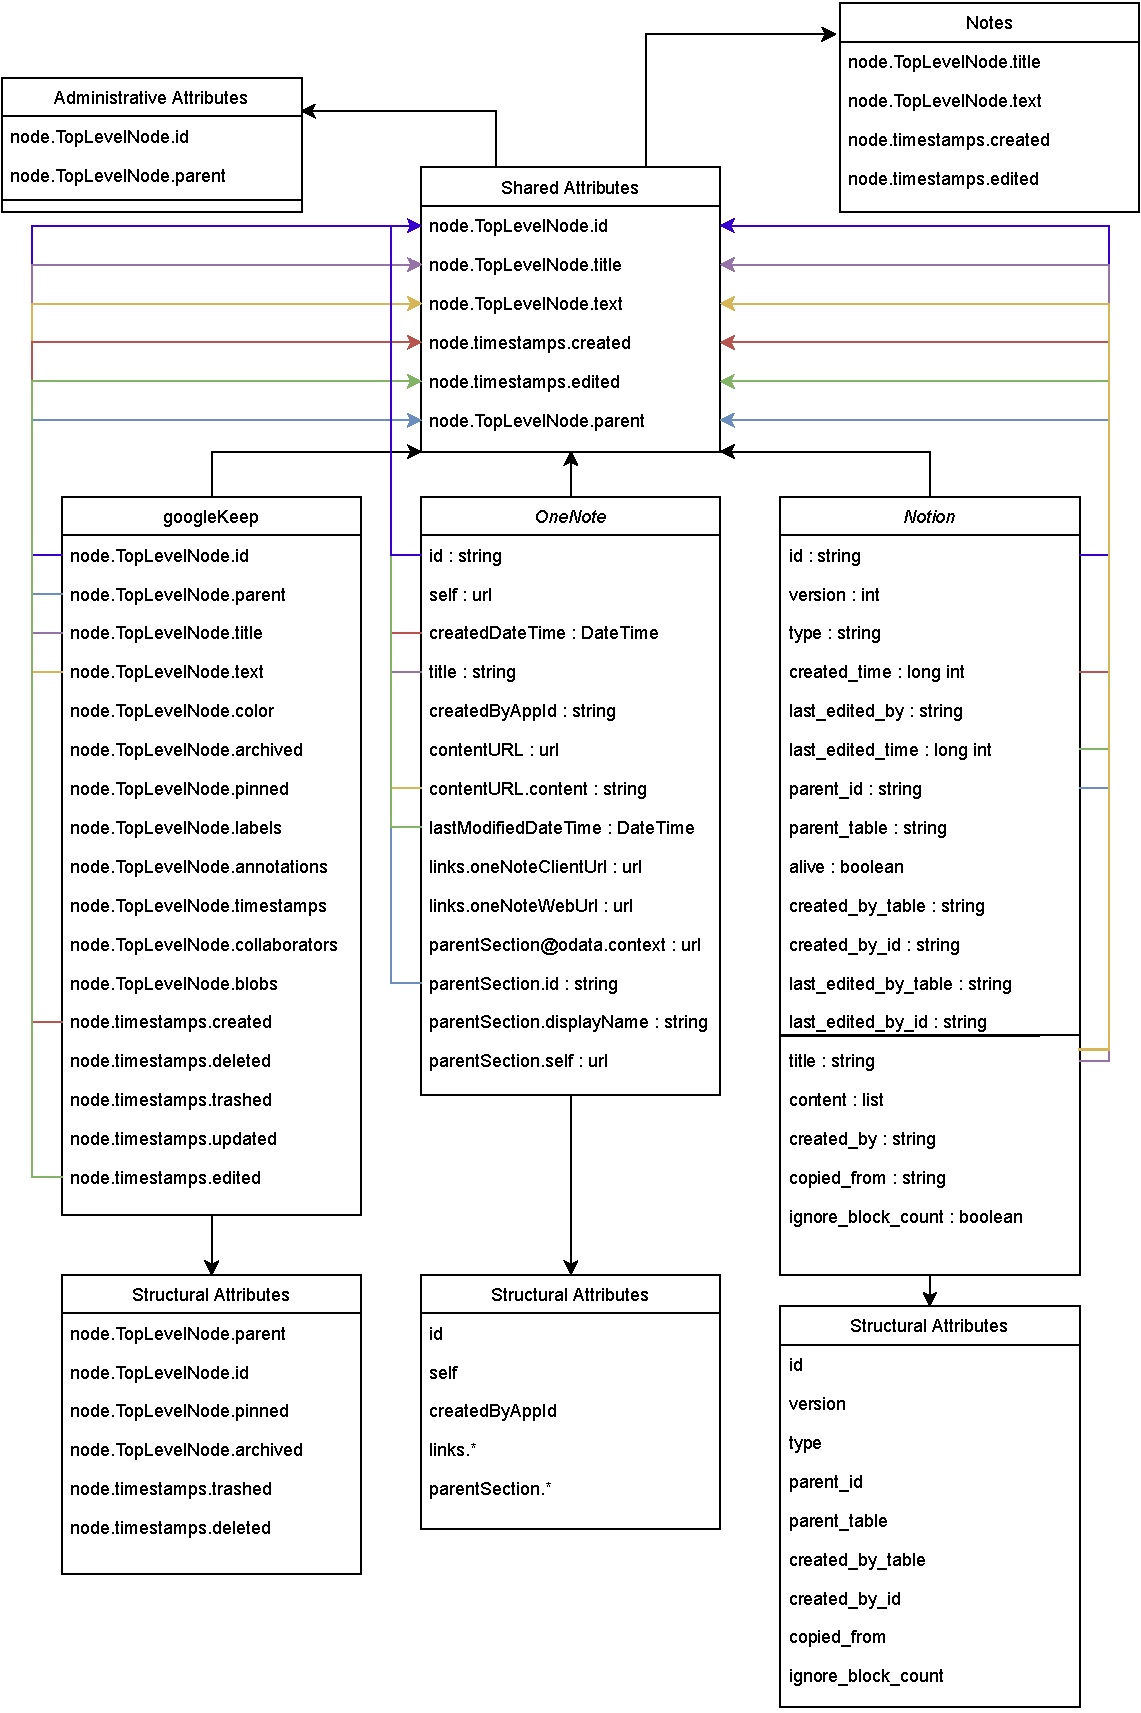
\includegraphics[width=1\textwidth]{Bilder/umsetzung/attributeUnion.pdf}
	\caption{Darstellung des Attribut-Vereinigungsprozesses}
	\label{fig:attrMatch}
\end{figure}
\clearpage

Nach der Vereinigung dieser Attribute mit denen aus den Kalender-Diensten wurden folgende Attribute in Tabelle \ref{tab:daten} für als feste, zwingend notwendige Eigenschaften eines jeden internen Datensatzes definiert. 

\begin {table}[H]
	\caption{Gemeinsame Attribute aller Dienste}
	\begin{tabular}{|l|l|l|}
		\hline
		\textbf{Wert} & \textbf{Datentyp} & \textbf{besondere Formatierung}\\
		\hline
		id & string & <Diensttyp>\#<Dienstklassenname>\#<Dienst-ID>\\
		title & string & \\
		text & string & \\
		created & string & <J>-<M>-<T>T<S>:<M>:<S>.<ZZ>Z (UTC-Zeitformat)\\
		edited & string & <J>-<M>-<T>T<S>:<M>:<S>.<ZZ>Z (UTC-Zeitformat)\\
		\hline
	\end{tabular}
	\label{tab:daten}
\end{table}

Jeder Datensatz aus den Anwendungen muss diese Attribute enthalten, um in die Datenbank aufgenommen zu werden. Die übrigen Eigenschaften, welche nicht in allen anderen Diensten enthalten sind, werden ebenfalls in die Datenbank übertragen. Bei diesen muss jedoch bei der Rückführung des Datensatzes in den Dienst die Existenz des Attributes geprüft werden. Existiert dieses nicht, wird diese Information bei der Injektion ausgelassen, wodurch die Schnittstelle einen Standardwert einfügt.

\section{Festlegung der Klassenstruktur}

Um sicherzustellen, dass die festen Attribute vorhanden sind, werden die Daten in einer Klasse statt einer Datenstruktur gespeichert. Dabei gibt es eine Basisklasse, welche die festen Attribute enthält, und mehrere abgeleitete Klassen mit den diensteigenen, optionalen Werten. Diese Klassen besitzten keine Methoden, da sie als reine Speicherklassen genutzt werden. Objekte dieser Klassen werden durch die Dienst-Schnittstellenklassen erstellt. Deren Aufgabe ist die Kommunikation mit den Diensten über deren jeweilige Benutzerschnittstellen. Sie übernehmen also die Anmeldung, die Extrahierung von Daten aus der Anwendung und die Injektion der Daten aus der Datenbank zurück in den Dienst. Sie fungieren außerdem als Bedienungsschnittstelle für die Nutzeroberfläche. Dabei werden auch hier alle Dienst-Schnittstellenklassen von einer Basis-Klasse abgeleitet, wodurch man sicherstellt, dass alle Unterklassen auf die gleichen Resourcen zugreifen und die gleiche Funktionalität bereitstellen. Die letzte Klassengruppe stellen die Datenbank-Schnittstellenklassen dar. Diese ermöglichen den Datentransfer zu und von der Datenbank. Ebenso wie bei den Dienst-Klassen, wird auch hier eine Vererbungsstruktur genutzt, um eine Konsistenz zwischen den abgeleiteten Klassen sicherzustellen. Das gesamte Konzept ist dabei auf hohe Flexibilität und Erweiterbarkeit ausgelegt. So kann ein neuer Dienst einfach über das Hinzufügen einer neuen Dienst-Klasse eingebunden und die Datenbank über eine neue Datenbank-Klasse gewechselt werden. In beiden Fällen sind entweder keine oder nur wenige Zeilen an Änderungen in den vorhanden Klassen nötig. Durch das vereinheitlichte Datenkonzept ist zudem eine hohe Kompatibilität gegeben. Eine Übersicht über die Klassenstruktur ist in Abbildung \ref{fig:Klassendiagram} zu sehen. Die Dienst-Klassen sind dabei die \textit{apiInterfaces}, die Datenbank-Klassen die \textit{datastores} und die Speicherklassen die \textit{dataObjects}. Die Zeit-Attribute haben den Datentyp \textit{string}, da zur Vereinheitlichung alle Zeitdatentypen in eine einheitlich formatierte Zeichenkette umgewandelt werden (zu sehen in Tabelle \ref{tab:daten}).\\

\begin{figure}[H]
	\centering
	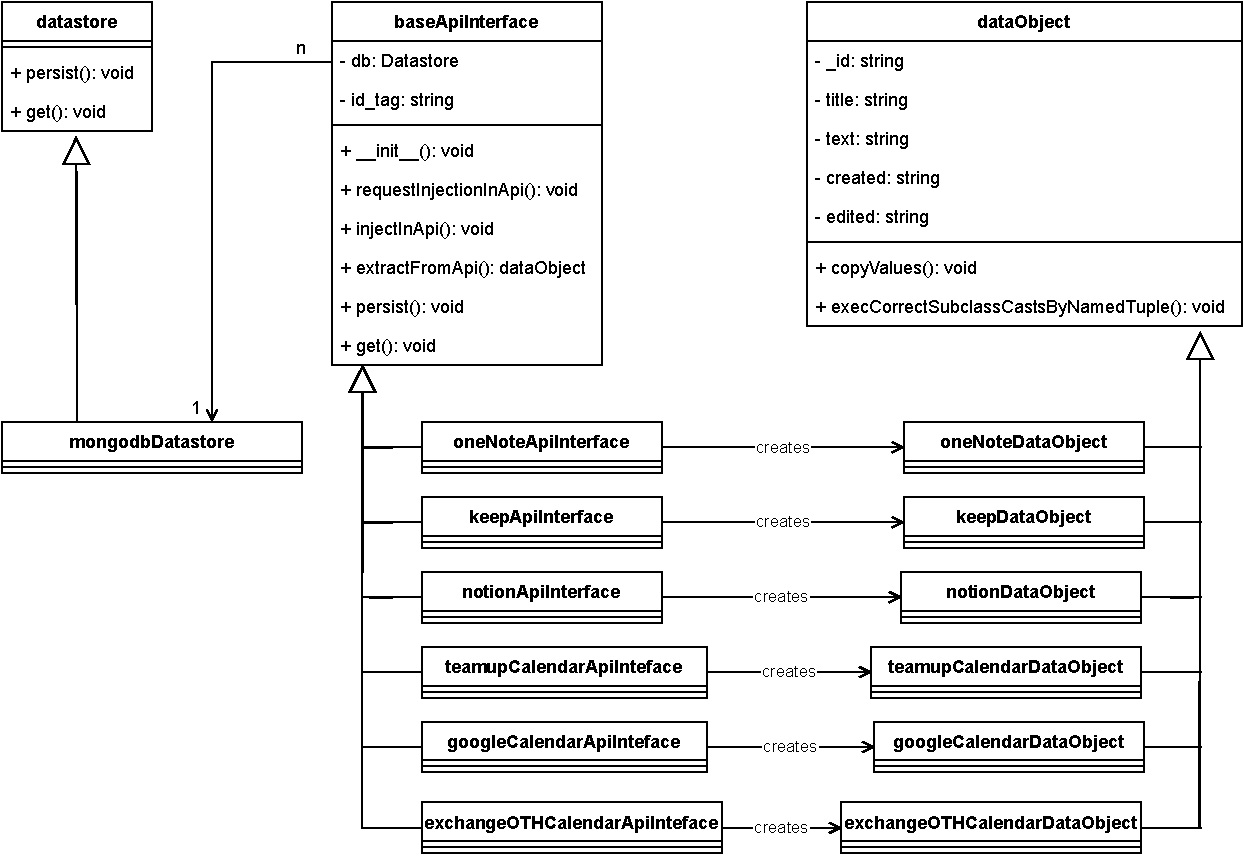
\includegraphics[width=1\textwidth]{Bilder/umsetzung/classDiagramm.pdf}
	\caption{Vereinfachtes Klassendiagramm zur Darstellung der Klassenstruktur}
	\label{fig:Klassendiagram}
\end{figure}

\section{Umsetzung des Speichervorganges}

Um ein Element aus der Anwendung zu extrahieren, muss dessen Benutzerschnittstelle angesprochen werden. Zuerst meldet sich die Schnittstellenklasse bei dem Dienst an und erhält ein Zugriffsobjekt. Bei den Notiz-Diensten wird mit diesem Objekt zuerst eine Suche nach allen vorhandenen Elementen gestartet und deren Attributwerte in die jeweilige Speicherklasse übertragen. Dabei wird die \textit{\_id} mit einem Präfix aus dem Diensttypen und der Ursprungsklasse versehen. Dies ist dann beispielsweise der Zusatz \textit{notes\#keepApiInterface\#} für den \textit{Keep-Dienst} des Unternehmens \textit{Google}. Zudem werden alle Zeitangaben auf das in Tabelle \ref{tab:daten} dargestellte Zeitformat konvertiert. Die Speicherung der Daten-Klasse übernimmt die Methode \textit{persist}. Diese nutzt das Attribut \textit{db} aus der Basisklasse, um die \textit{persist}-Methode aus der Datenbank-Klasse aufzurufen. Im Prototyp ist dies der \textit{mongodbDatastore}. Dieser wiederum stellt eine Verbindung zur Datenbank her und erhält dessen Verbindungsobjekt. Die Speicherklasse wird in eine \textit{dict}-Speicherstrucktur umgewandelt und in den Dienst eingefügt. Es wird also eine Sammlung von Schlüssel-Werte-Paaren übergeben. Die Konvertierung ist dabei im Falle des \textit{mongodbDatastores} nötig, da die Verbindungsklasse keine Klassen als Eingabeparameter akzeptiert und eine Konvertierung in ein \textit{dict} leicht zu realisieren ist. Die Injektion in die Datenbank findet mithilfe der \textit{replace\_one()}-Methode von \textit{MongoDB} statt. Dabei ist die \textit{upsert}-Option gesetzt, um sicherzustellen, dass nicht vorhandene Einträge eingefügt werden. Existieren diese bereits, ersetzt die Methode sie durch den neuen, übergebenen Eintrag, was einer Aktualisierung gleichkommt.

\section{Definition des Extraktionsvorganges aus der Datenbank und der Datenrückführung in einen Dienst}

Der Rückweg aus der Datenbank in die Dienste beginnt dabei ebenfalls in den Schnittstellenklassen. Die Notiz-Klassen bereiten in der Methode \textit{requestInjection} die Ergebniszähler vor und rufen die Methode \textit{requestInjectionInApi} auf. Dessen Parameter stammen dabei aus den übergebenen Werten der aufrufenden Methode. Diese haben dabei auch Standartwerte, welche dem Nutzer eine selektierte Angabe ermöglichen. Die Parameter sind in Tabelle \ref{tab:params} mit ihrem Datentypen und ihrer Bedeutung aufgelistet.

\begin {table}[H]
\caption{Parameter der Methoden zur Rückholung der Daten aus der Datenbank}
\begin{tabular}{|l|l|p{6.2cm}|}
	\hline
	\textbf{Parameter} & \textbf{Datentyp} & \textbf{Bedeutung}\\
	\hline
	substrIdTag & String & Stellt den Präfix dar, nach welchem die \_id-Felder in der Datenbank gefiltert werden sollen. \\
	\hline
	filterOptions & Liste aus \textit{Dictionaries} & Enthält die zusätzlichen Filteroptionen für die MongoDB Aggregationsmethode.\\
	\hline
	transformationOptions & Liste aus \textit{Dictionaries} & Enthält die Datentransformationsinformationen für die MongoDB Aggregationsmethode. Beispielsweise werden Werte geändert oder Variablenwerte anderen Variablen zugewiesen.\\
	\hline
	addAggOptions & Liste aus \textit{Dictionaries} & Damit können weitere MongoDB Parameter für die Aggregationsmethode angegeben werden. Beispielweise ist durch eine Angabe des \textit{\$unset}-Befehls eine Löschung eines Feldes möglich.\\
	\hline
\end{tabular}
\label{tab:params}
\end{table}

Die Methode \textit{requestInjectionInApi} aus der Basis-Klasse leitet diese wiederum an die \textit{get}-Methode der Datenbank-Klasse weiter. Jedoch kommt hier der Parameter \textit{serviceObject} hinzu, welcher einfach eine Referenz auf das aufrufende Objekt - also die Schnittstellenklasse - ist. Die aufgerufene Methode des \textit{mongodbDatastore} stellt dann zuerst eine Verbindung zur Datenbank her und definiert aus den übergebenen Werten eine \textit{Aggregation Pipeline}. Damit werden die Daten nach den angegebenen Optionen gefiltert, transformiert oder anders verändert und an die Datenbank-Klasse als \textit{Dictionary} zurückgegeben. Für jeden Eintrag in dieser Wertesammlung wird nun die \textit{injectInAPI}-Methode der aufrufenden Schnittstellen-Klasse über die übergebene Referenz aufgerufen. Diese meldet sich bei dem jeweiligen Dienst an und überprüft zuerst, ob die \textit{id} aus dem Eintrag schon im Dienst vorhanden ist. Ist das der Fall, werden die Einträge aktualisiert. Wenn nicht, wird dieser als neuer Eintrag eingefügt. Die zusätzlichen Attribute, welche in den abgeleiteten Klassen von \textit{dataObject} gespeichert werden, müssen dabei auf Existenz überprüft werden, da die Einträge auch von anderen Diensten stammen können. Eine weitere Aufgabe ist die Registrierung und das Abfangen von Fehlern bei der Injektion. Entsteht ein Fehler wird dieser abgefangen, ausgeben und die Variable \textit{errorCount} inkrementiert. Kann der Eintrag problemlos verarbeit werden, erhöht sich die Variable \textit{successCount}. In der Klasse \textit{oneNoteApiInterface} ergibt sich dabei eine Besonderheit. Da der Dienst nur eingeschränkte Änderungen an den Einträgen zulässt, wird bei Erkennen eines Eintrages im Dienst die letzte Änderungszeit überprüft. Ist der Eintrag im Dienst jünger als der in der Datenbank wird die Variable \textit{ignoredCount} inkrementiert und der Eintrag übersprungen. Andernfalls wird dieser neu eingefügt und als Erfolg gezählt. Nachdem alle Einträge eingefügt oder aktualisiert wurden, gibt die Ursprungsmethode \textit{requestInjection} noch die Variablen \textit{errorCount}, \textit{ignoredCount} und \textit{successCount} als Ergebnis aus. In Abbildung \ref{fig:bspInj} ist die Ausgabe auf der Konsole für den gesamten Injektonsprozess zu sehen. 

\begin{figure}[H]
	\centering
	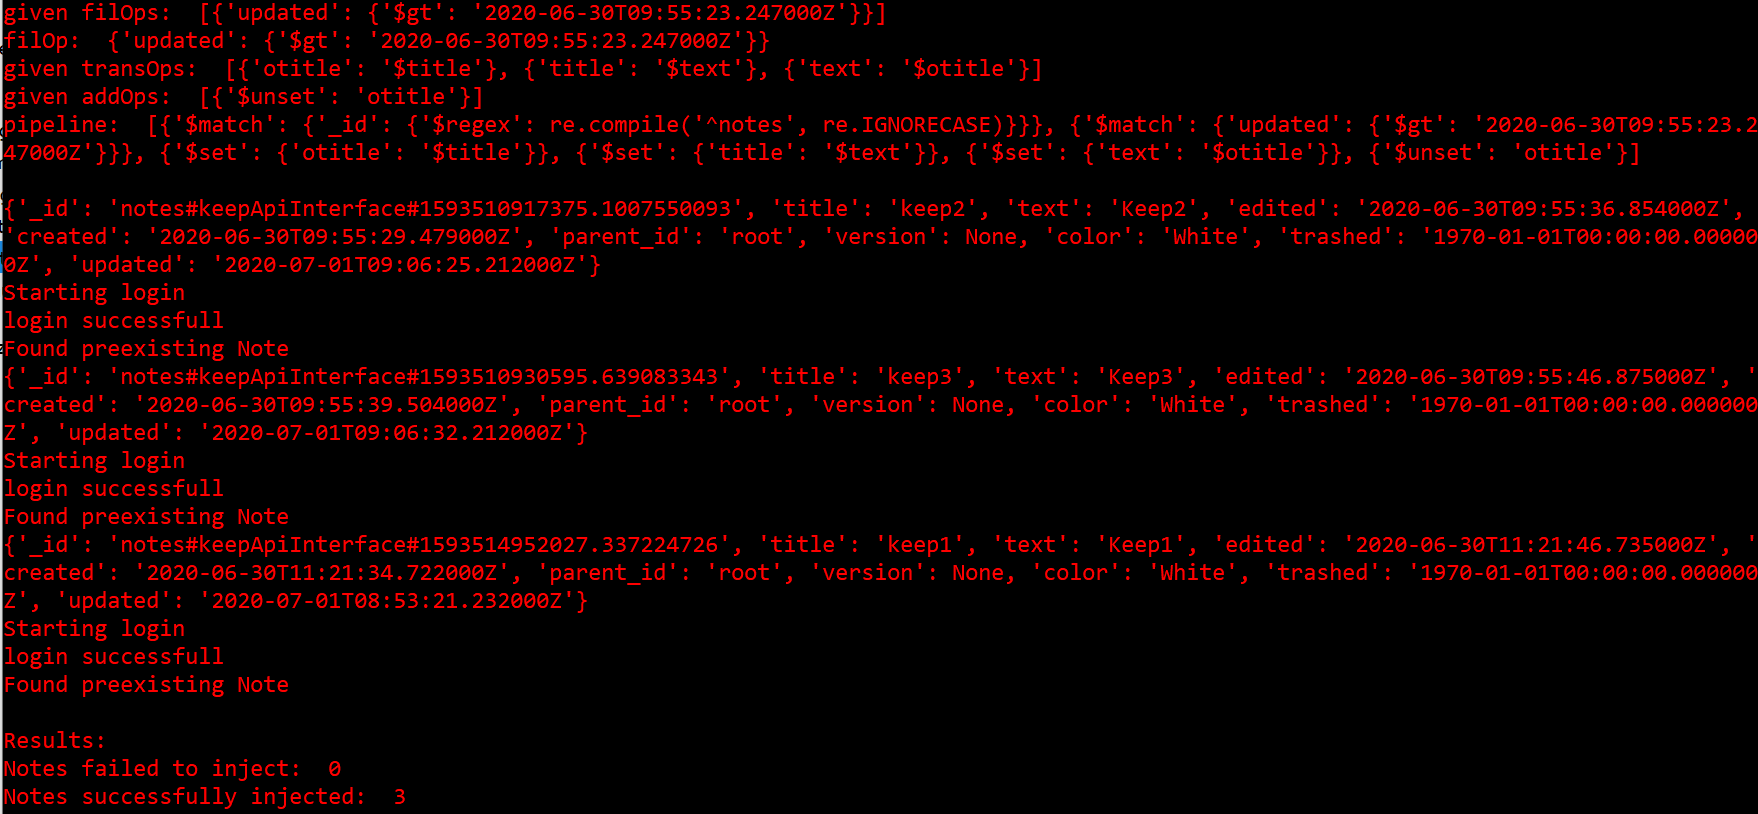
\includegraphics[width=1\textwidth]{Bilder/umsetzung/BeispielInject.png}
	\caption{Konsolenausgabe für den Injektionsvorgang}
	\label{fig:bspInj}
\end{figure}

\newpage
\section{Aufbau der grafischen Oberfläche}

Bedient wird das System über eine einfache \textit{Python} Benutzeroberfläche. Diese besteht aus der Auswahl der Dienste für Eingabe und Ausgabe der Daten, sowie der Selektion und Zuordnung von deren Attributen. In Zweiteren kann auch den Attributen des Eingabedienstes eine anderes Attribut des Ausgabedienstes oder ein fester, eigener Wert zugewiesen werden. Diese Konfigurationen stellen dann die Parameter aus Tabelle \ref{tab:params}, welche für die \textit{pipeline} in der Datenbankklasse genutzt werden. Die Auswahl in den einzelnen Felder findet über ein \textit{Drop-Down} Menü statt. Bei den Attributen kann auch eine eigener Wert eingetragen werden. Zu sehen ist die Oberfläche in Abbildung \ref{fig:gui}. 

\begin{figure}[H]
	\centering
	%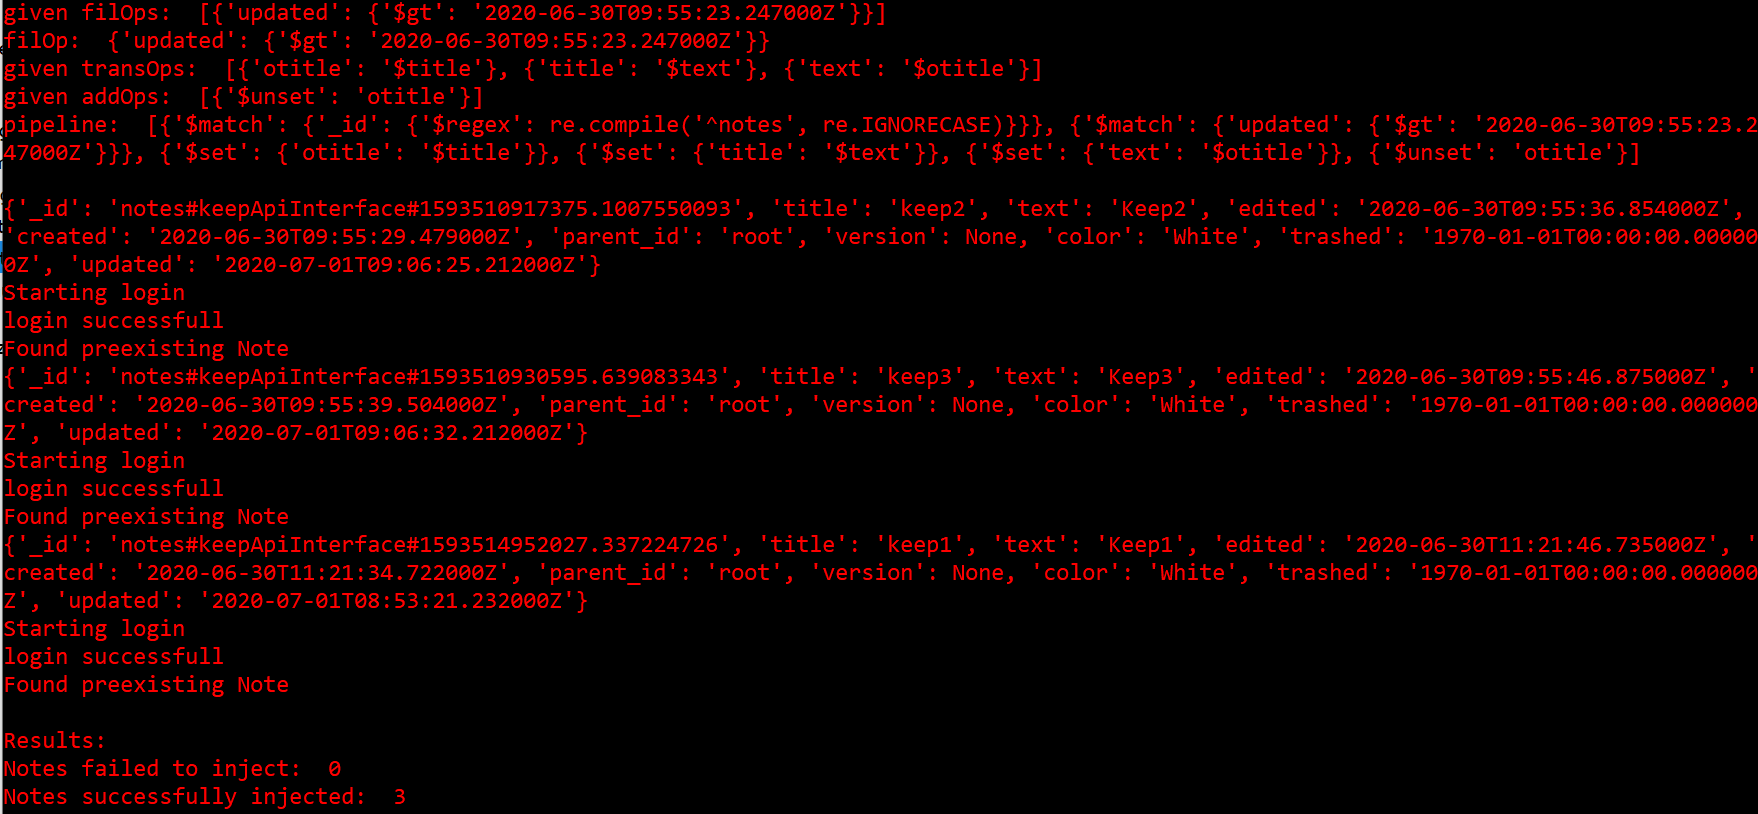
\includegraphics[width=1\textwidth]{Bilder/umsetzung/BeispielInject.png}
	\caption{Graphische Oberfläche des Systems}
	\label{fig:gui}
\end{figure}